\documentclass[ a4paper,
                oneside,
                toc=bibliography,
                toc=listof
                ]{scrbook}

\usepackage[ngerman]{babel} % If the thesis is in English
\usepackage {longtable}
%\usepackage[english, ngerman]{babel} % If the thesis is in German


% This class does the ISW styling for you (together with scrbook).
%
% It handles the following:
% - Proper input and font encoding (Just type, don't care about the LaTeX compiler you use or how to type German umlauts)
% - Fonts with ligatures and kerning (Tex Gyre fonts are used, part of every LaTeX installation, text is nice to read)
% - Bibliography styling for biblatex (declare your bibliography file and you are ready to go)
% - Provide command for title page (\makeISWtitle) and declaration of originality ( \declarationOfOriginality)
% - Loads packages "biblatex" and "graphics"
\usepackage[
    type=study, % master, bachelor, bachelorproject
]{iswthesis}

%Path to .bib-File(s) for BibLatex
\addbibresource{bibliography.bib}
% \addbibresource{someOtherBibFile}

\author{Lukas Schlotter}
\placeOfBirth{Stuttgart}
\major{Mechatronik}
\title{Konzeption und Implementierung einer Diagnoseschnittstelle zwischen Industrieroboter und Anlagensteuerung}
\titleTranslated{Design and Implementation of a Diagnostic Interface between Industrial Robot and Control System}
\matrnr{3668915}
\date{\today}
\supervisor{Dr.-Ing. Andreas Wolf, Dipl.-Ing. Daniel Knauss}
\professor{Prof. Dr.-Ing. Alexander Verl}

\begin{document} 
    \frontmatter
    \makeISWtitle
    
    \cleardoublepage
	\setcounter{page}{1} % start at page (i) after title page
    %\declarationOfOriginality

    % Kurzfassung/Abstract
    
    \cleardoublepage
    \tableofcontents
    

    \mainmatter
    
    \chapter{Einleitung}

    \section{Motivation}
    

    
    \begin{table}[h!]
    	\centering
    	\begin{tabular}{||c c c c||} 
    		\hline
    		Col1 & Col2 & Col2 & Col3 \\ [0.5ex] 
    		\hline\hline
    		1 & 6 & 87837 & 787 \\ 
    		2 & 7 & 78 & 5415 \\
    		3 & 545 & 778 & 7507 \\
    		4 & 545 & 18744 & 7560 \\
    		5 & 88 & 788 & 6344 \\ [1ex] 
    		\hline
    	\end{tabular}
    	\caption{Table to test captions and labels.}
    	\label{table:1}
    \end{table}
	
	\section{Anforderungsdefinition / Aufgabenstellung}
	
	\section{Methodik und Vorgehensweise}
	Die Verwendung geeigneter Methoden und eines strukturierten Vorgehens sind entscheidend für eine erfolgreiche Umsetzung des Projektes. Durch ein Vorgehensmodell wird eine effiziente Arbeitsweise und eine zeitgerechte Fertigstellung gefördert. Da die Komplexität des Projektes und der Software im Projektverlauf zunehmend wächst, ist eine wissenschaftliche Methodik essentiell. Methoden und Werkzeuge erleichtern es neue Lösungsansätze zu finden und faktenbasierte Entscheidungen zu treffen. \cite{SoftwaretechnikBroy} \cite{ISWLeitfaden}
	Gant-Diagramm wie Seite 39 ISW-Leitfaden

	\chapter{Grundlagen und Stand der Technik}
	
	\section{Feldbusse}
	Maschinen und Anlagen verfügen über eine Vielzahl an Sensoren und Aktoren. Diese werden klassisch über Parallelverdrahtung an die Ein-und Ausgänge der SPS angeschlossen. Ein Feldbus ermöglicht es dagegen die Sensoren und Aktoren an einzelne aktive Verteilerboxen anzuschließen. Die Verteilerboxen werden wiederum mit einem Feldbus untereinander und mit der SPS verbunden. Dies ermöglicht eine Dezentralisierung, was den Schaltschrank vereinfacht, die Energieeffizient steigert und die Flexibilität bezüglich Änderungen erhöht. Der Übergang von der Parallelverdrahtung zu der Fehlbusverdrahtung ist mit den Zwischenschritt von passiven Verteilerboxen nachfolgend dargestellt (vgl. Abbildung \ref{fig:Parallel_vs_Feldbus}). Bei der Feldbus Anschaltung wird meist wie in der Abbildung dargestellt eine Linien-Struktur verwendet. Alternativen sind die Stern-, Ring- oder Baum-Struktur. \cite{hering2012elektrotechnik}
	\begin{figure}[!ht]
		\centering
		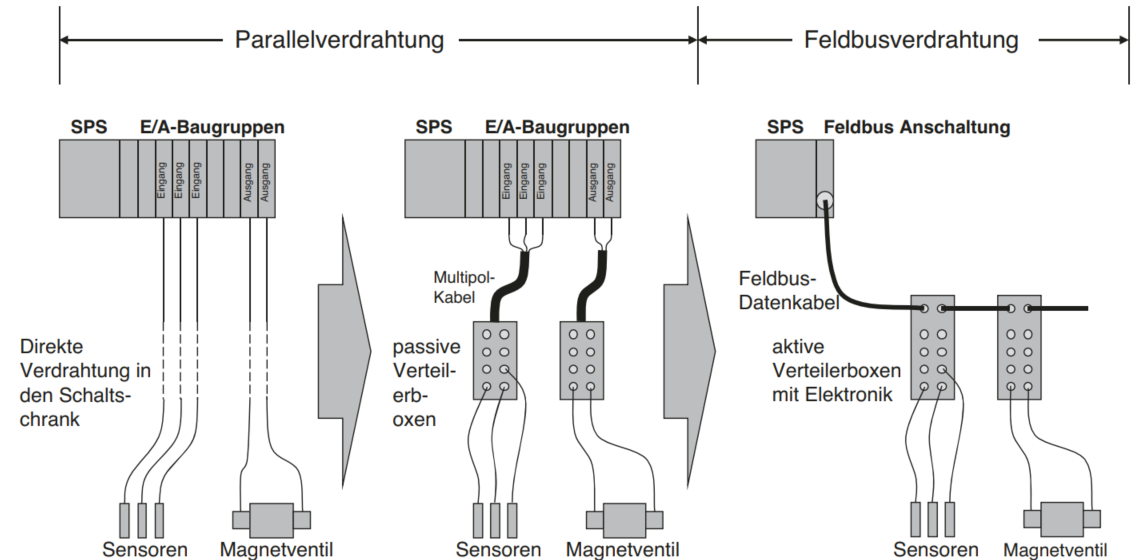
\includegraphics[width=1.0\linewidth]{./images/Parallelverdrahtung_Feldbus.png}
		\caption{Übergang Parallelverdrahtung zu Feldbussen \cite{hering2012elektrotechnik}}
		\label{fig:Parallel_vs_Feldbus}
	\end{figure}\\
	Es haben sich Feldbusse von vielen namhaften Herstellern etabliert. Mittlerweile werden diese Standard-Feldbusse immer weiter von Ethernet basierenden Feldbussen (auch Industrial Ethernet genannt) abgelöst, da diese vor allem Vorteile bezüglich der Übertragungsgeschwindigkeit aufweisen. Die Marktaufteilung aus dem Jahr 2021 ist nachfolgend abgebildet, wobei eine weitere Zunahme der Marktanteile von den Ethernet basierenden Feldbussen zu erwarten ist (vgl. Abbildung \ref{fig:Marktanteil_Feldbus}). \cite{hering2012elektrotechnik} \cite{Marktanteile_HMS}\\
	\begin{figure}[!ht]
		\centering
		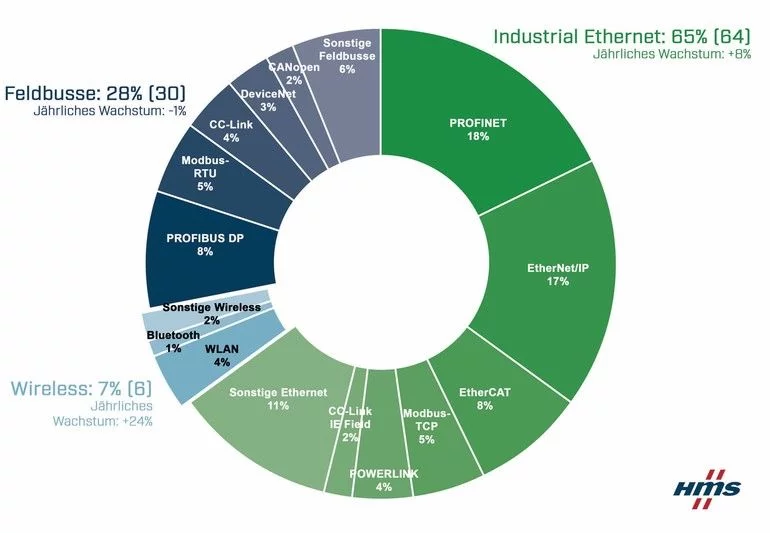
\includegraphics[width=1.0\linewidth]{./images/HMS__Marktanteile_industrielle_Netzwerke.png}
		\caption{Marktanteile Feldbusse und Industrial Ethernet  \cite{Marktanteile_HMS}}
		\label{fig:Marktanteil_Feldbus}
	\end{figure}\\
	
	\subsection{Standard-Feldbusse}
	In der Anlagentechnik und der Robotik ist die sofortige zuverlässige Datenübertragung unter anderem aus Gründen der Sicherheit essentiell. Feldbusse sind daher echtzeitfähig. Die Echtzeitfähigkeit besagt, dass die Daten innerhalb einer sehr kurzen festgelegten Zeitspanne unabhängig von äußeren Einflüssen übertragen werden müssen. Durch die harte Echtzeit, ist im Gegensatz zur weichen Echtzeit zusätzlich definiert, dass die Daten mit einem absoluten Determinismus übertragen werden müssen. Bei der weichen Echtzeit verlieren die Daten lediglich an Nutzen bei verspätetem Eintreffen, bei der harten Echtzeit werden sie komplett nutzlos. Aus diesem Grund müssen bei der harten Echtzeit 100 \% der Daten innerhalb der definierten Zeit übertragen werden, was insbesondere bei sicherheitsrelevanten Funktionen von Relevanz ist. \cite{dopatka2008framework} \cite{Echtzeit} \\
	Im folgenden sollen ein paar gängige Feldbusse kurz erwähnt und erläutert werden.\\
	\textbf{Profibus} wird von dem Dachverband "Profibus \&Profinet" International" verwaltet, um die Interessen der Nutzer einzubringen. Neben dem Profibus auf Feldbus-Ebene (auch Profibus-DP genannt) existiert eine weitere Variante auf Zellensteuerungs-Ebene und eine auf Prozess-Automatisierungs-Ebene. Als Übertragungstechnik dient der sogenannte RS485-Standard mit einer Zweidrahtleitung. Die Datentransferrate von Profibus beträgt bis zu 12 MBit/s. Speicherprogrammierbare Steuerungen von Siemens setzen häufig Profibus ein.  \cite{hering2012elektrotechnik}\\
	\textbf{CAN-Bus} wurde ursprünglich für die Automobil-Industrie entwickelt und kommt dort heute noch zum Einsatz. Darüber hinaus, nahm die Verbreitung in der Anlagensteuerung zu. Möglich sind Datentransferraten von bis zu 1 MBit/s. Als Übertragungsmedium dient eine Zweidrahtleitung.  CAN-Bus zeichnet sich durch eine besonders hohe Datensicherheit, also eine hohe Zuverlässigkeit bei der Datenübertragung aus, weshalb er in der Medizintechnik und Robotik hohen Zuspruch findet. \cite{hering2012elektrotechnik}\\
	\textbf{DeviceNet} basiert auf CAN und ist eine Entwicklung des nordamerikanischen Herstellers "Rockwell Automation". Die Datenübertragungsrate beträgt bis zu 500 kBit/s und die Spannungsversorgung, sowie die Datenkommunikation können über ein Kabel erfolgen. \cite{hering2012elektrotechnik}\\
	\textbf{CC-Link} stellt eine Entwicklung des Unternehmen Mitsubishi dar. Verwaltet wird das Protokoll von einer Anwenderorganisation ähnlich zu Profibus. Die maximale Übertragungsrate beträgt 10 MBit/s und als Übertragungsmedium dient eine dreiadrige Leitung. \cite{hering2012elektrotechnik}\\
	\label{subsec:StandardFeldbus}
	\subsection{Ethernet basierende Feldbusse}
	Ethernet basierende Feldbusse, häufig auch als "Industrial Ethernet" bezeichnet, ermöglichen deutlich höhere Übertragungsraten als Standard-Feldbusse. Daher nimmt deren Verbreitung ständig zu und lösen in vielen Bereichen den Standard-Feldbus ab. \cite{hering2012elektrotechnik}\\
	\textbf{Ethernet-Technologie}\\
	Ethernet ist einer von mehreren Standards für die lokale Netzwerkverbindung mittels LAN-Technologie. Sie ist im IEE 802-3- Standard (Institute of Electrical and Electronis Engineers) genormt. Der Aufbau eines Ethernet-Telegramms ist nachfolgend abgebildet (vgl. Abbildung \ref{fig:EthernetTelegramm}). Die Adressierung erfolgt mittels MAC-Adresse oder IP-Adresse (mehr hierzu in Kapitel \ref{sec:TCP/IP}). \cite{riggert2002rechnernetze}\\
	\begin{figure}[!ht]
		\centering
		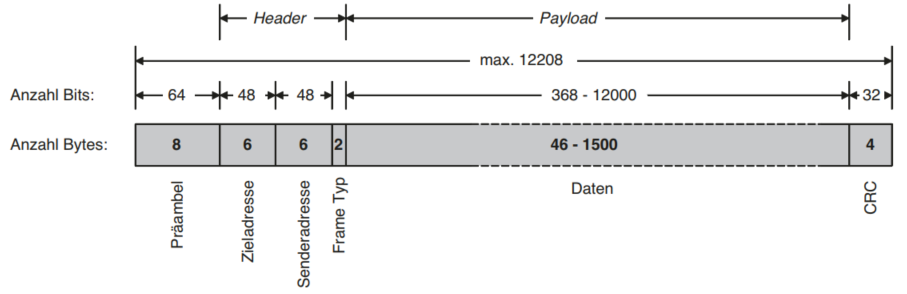
\includegraphics[width=1.0\linewidth]{./images/Ethernet-Telegram.png}
		\caption{Telegramm-Aufbau Ethernet \cite{hering2012elektrotechnik}}
		\label{fig:EthernetTelegramm}
	\end{figure}
	Verschiedene Geräte sind an das Übertragungsmedium angeschlossen und teilen sich dieses. Man spricht von einem Multi-Master-Bus, da jedes Gerät selbständig die Initative ergreifen kann, um Nachrichten zu senden. Damit jedes Gerät kommunizieren kann und dabei Sendekonflikte vermieden werden kommt bei Ethernet der CSMA/CD-Mechanismus zum Einsatz. CSMA/CD steht für "Carrier Sense Multiple Access with Collision Detection" und ermöglicht einen mehrfachen Zugriff (Muliple Access) auf das Übertragungsmedium. \cite{hering2012elektrotechnik} \cite{riggert2002rechnernetze}
	\begin{itemize}
		\item \textbf{Carrier Sense:} Es überwacht, dass das Übertragungsmedium nicht durch ein anderes Gerät belegt ist. Erst nachdem das Medium als frei erkannt wird, erfolgt nach einer kurzen Wartezeit die Übertragung. Während des Sendens, wird das Medium weiterhin auf Kollisionen abgehört.
		\item \textbf{Multiple Access:} Es besagt, dass alle Geräte gleichberechtigt auf das Übertragungsmedium zugreifen können.
		\item \textbf{Collision Detection:} Wenn mehrere Geräte zur gleichen Zeit das Übertragungsmedium als frei erkennen kommt es zur Überlagerung, da mehrere Geräte gleichzeitig beginnen zu senden. Dies wird als Kollision bezeichnet und es kommt zur Signalverfälschung durch Überlagerung. Da jeder Sender das Übertragungsmedium während des Sendevorgangs überwacht wird die Kollision direkt erkannt. Dasjenige Gerät, welches die Kollision erkennt, informiert alle anderen Geräte mittels eines Signales über die aufgetretene Kollision und fordert diese zur Unterbrechung jeglicher Übertragung auf. \\
		Danach warten die Geräte eine zufällige Zeitspanne ab und versuchen das Senden erneut. \cite{riggert2002rechnernetze}
	\end{itemize}
	Durch die Kollisionen kommt es zu nicht vorhersehbaren Wartezeiten im Sendeprozess. Daher handelt es sich um ein nicht deterministisches Zugriffsverfahren. Ethernet mit CSMA/CD ist nicht echtzeitfähig, was wie bereits in Kapitel \ref{subsec:StandardFeldbus} erwähnt, zu Problem bei Automatisierungsanlagen führen kann.\\
	Um die Ethernet-Technologie dennoch in der Automatisierung zu nutzen, haben die Hersteller verschiedene Echtzeitprotokolle entwickelt, um Ethernet echtzeitfähig zu machen. Beispielsweise wird die Methodik CSMA/CD außer Kraft gesetzt und stattdessen durch sogenanntes Pooling oder ein Zeitscheibenverfahren ersetzt. Jeder Hersteller geht hier jedoch seinen eigenen Weg.	Bekannte Ethernet basierende Feldbusse sind Profinet, Ethernet/IP, EtherCAT und Sercos III.
	EtherCAT ist eine Technologie des Herstellers "Beckhoff", dessen SPS im Rahmen dieses Projektes zum Einsatz kommt. Aus diesem Grund ist EtherCAT die bevorzugte Technologie und wird im Rahmen dieser Arbeit näher erläutert. \cite{ethercat} \cite{riggert2002rechnernetze}\
	\\
	Weiterhin ist zu beachten, dass die Netzwerktopologie sich bei den Ethernet basierenden Feldbussen häufig von den Standard-Feldbussen unterscheidet. Während bei den Standard-Feldbussen die Ansteuerung vorwiegend in der Linienstruktur erfolgt, wird bei der Ethernet Anschaltung oft eine Sternstruktur mit einem Switch eingesetzt (vgl. Abbildung \ref{fig:TopologieEthernet}).
	\begin{figure}[!ht]
		\centering
		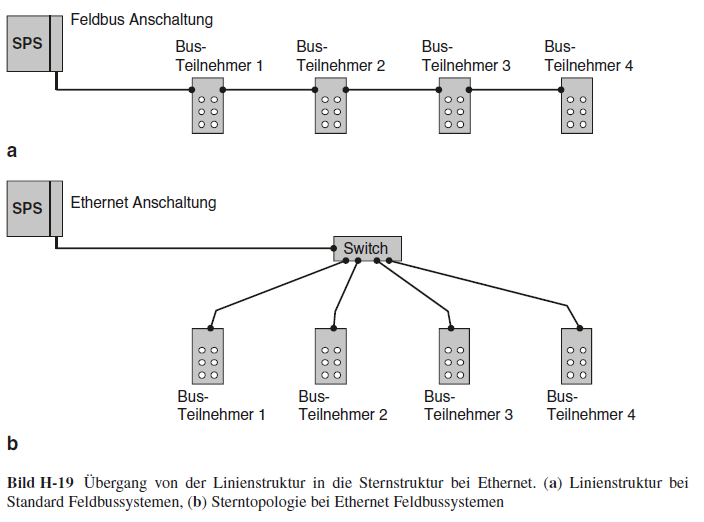
\includegraphics[width=1.0\linewidth]{./images/Feldbus vs Ethernet Anschaltung.png}
		\caption{Topologie: oben Standard-Feldbus, unten Ethernet basierender Feldbus \cite{hering2012elektrotechnik}}
		\label{fig:TopologieEthernet}
	\end{figure}\\
	Der Ethernet Switching Hub, abgekürzt als Switch erlernt beim Einschalten an welchen Ports  Teilnehmer angeschlossen sind. Der Switch leitet ein Datentelegramm eindeutig vom Sender zum Empfänger. Dadurch werden von dem Telegramm nicht betroffene Teilnehmer und Ethernet-Segmente nicht unnötig belastet und Kollisionen vermieden. Das Weiterschalten erfolgt auf Basis der Sende- und Ziel-Adresse, welche im Ethernet-Telegramm hinterlegt ist. \cite{hering2012elektrotechnik} \\
	\textbf{EtherCAT} \\
	Wie bereits erwähnt setzen viele Hersteller auf das Zeitscheibenverfahren oder Pooling, um EtherNet echtzeitfähig zu machen. Der Zeitverzug ist hierbei jedoch implementierungsabhängig und kann durch erforderliche technische Komponenten am Bus weiter steigen. Um dies zu verhindern setzt EtherCAT auf einen anderen Lösungsansatz. Im Gegensatz zu anderen Verfahren sollen Daten nicht mehr empfangen, interpretiert und dann wieder weiterversendet werden. Stattdessen setzt EtherCAT auf sogenannte FMMU (Fieldbus Memory Management Unit) in allen E/A-Klemmen. Diese FMMU entnimmt nur die relevanten Daten vom Bus, sodass die Telegramme mit einer Verzögerung von nur wenigen Nanosekunden weiterlaufen können. Zum Versenden werden Daten in die durchlaufenden Telegramme eingefügt, sodass es auch hier zu kaum einer Verzögerung kommt. Dieses Prinzip ist nachfolgend dargestellt (vgl. Abbildung \ref{fig:EtherCAT}).
	\begin{figure}[!ht]
		\centering
		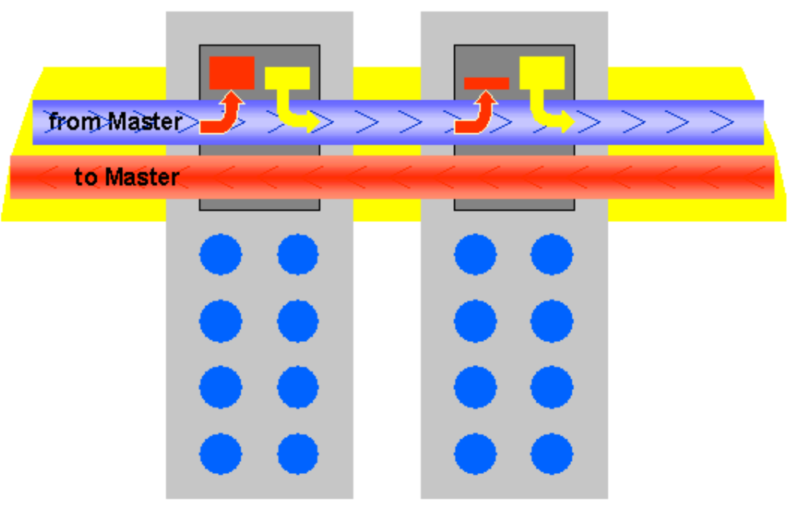
\includegraphics[width=0.7\linewidth]{./images/EtherCAT.png}
		\caption{Telegrammbearbeitung \cite{ethercat}}
		\label{fig:EtherCAT}
	\end{figure}\\
	Dabei wird auf dem gesamten Bus vom Ethernet-Protokoll nach IEEE 802.3 nicht abgewichen. Bit-Fehler werden so durch die CRC-Prüfsumme erkannt. Neben der Stern-Topologie unterstützt EtherCAT auch eine Linien- oder Baum-Struktur und viele weitere.
	EtherCAT zeichnet sich durch geringe Laufzeitverzögerungen und eine hohe Datenrate aus. Beispielsweise können 1000 E/as in nur 30 \(\mu s\) aktualisiert werden und auch eine Übertragungsrate GBit-Bereich ist mit Erweiterung möglich. \cite{ethercat}\\
	Multi-Master Bussen (z.B. CAN oder TCP/IP) vs. Mono-Master
	
	\section{TCP/IP}
	TCP/IP (Transmission Control Protocol/Internet Protocol) ist das meist verwendete Netzwerkprotokoll weltweit und zudem frei zugänglich. Durch dieses Protokoll wird definiert, wie Daten durch Netzwerkkommunikationshardware versendet und empfangen werden kann. Welches Übertragungsmedium verwendet wird ist  nicht definiert, sodass sich neben LAN z.B. auch WLAN einsetzen lässt.\cite{CS9_TCP} \cite{kim2016service} \\
	TCP/IP ist nicht echtzeitfähig, stellt jedoch eine gute Ergänzung zu den Echtzeitprotokollen dar, um nicht zeitkritische Daten, wie z.B. zur Diagnose oder  Visualisierung zu übertragen. Bei TCP/IP handelt es sich um eine sichere Datenübertragung die Nachrichten in einen Bytestrom verpackt und entpackt. Vom Sender zum Empfänger durchlaufen die Daten vier Schichten (vgl. Abbildung \ref{fig:Schichtenmodell}). Für eine sichere fehlerfreie Übertragung werden die eigentlichen Daten ergänzt um die MAC-/IP- und TCP-Header. Das CRC-Feld stellt eine Art Prüfsumme, mit welcher die Korrektheit der übertragenen Daten überprüft wird. \cite{hering2012elektrotechnik}
	\begin{figure}[!ht]
		\centering
		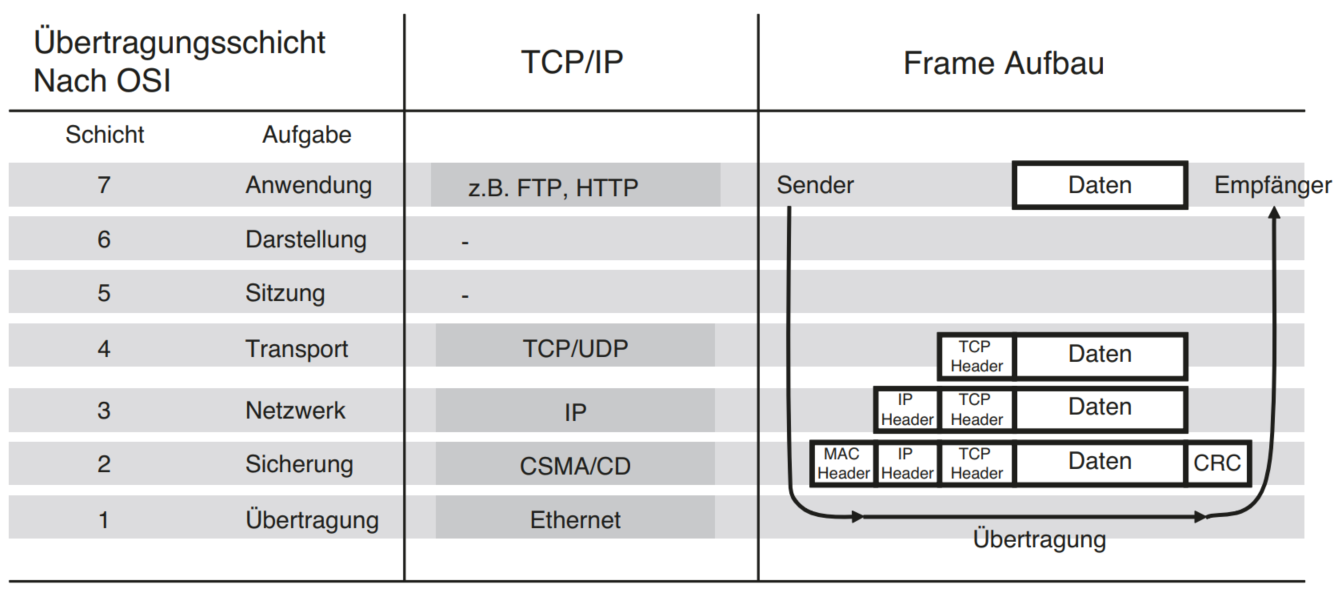
\includegraphics[width=1.0\linewidth]{./images/Schichtenmodell_TCP_IP.png}
		\caption{Schichtenmodell TCP/IP \cite{hering2012elektrotechnik}}
		\label{fig:Schichtenmodell}
	\end{figure} \\
	TCP/IP setzt sich aus den Protokollen TCP und IP zusammen.\\
	\\
	\textbf{TCP}\\
	Das Ziel von TCP ist eine fehlerfreie Datenübertragung. Hierzu muss der Empfänger die korrekt erhaltenen Daten, über eine Nachricht, die an den Sender zugesendet wird, bestätigen. Die Überprüfung der Korrektheit erfolgt mit dem CRC-Segment. Erhält dieser Sender diese Bestätigung nicht wird erneut versucht die Daten zu versenden. Hierdurch ist eine fehlerfreie und lückenlose Datenübertragung, selbst bei Netzwerkproblemen garantiert, was jedoch die Prozesse verlangsamt. Eine Alternative zu TCP ist UDP (User Datagram Protocol) . Hierbei erhält der Absender keine Bestätigung, dass die Daten korrekt empfangen wurde. Der Sender fährt direkt mit der Versendung der nächsten Pakete durch. Eine fehlerfreie Übertragung ist nicht garantiert, jedoch ist sie im Vergleich zu TCP schneller. Sowohl TCP, als auch UDP bauen auf dem Internetprotokoll IP auf. \cite{CS9_TCP}\\
	\\
	\textbf{IP} \\
	Das IP-Protokoll arbeitet auf der Internet bzw. IP-Schicht des TCP/IP-Protokolls, was der Netzwerkschicht des OSI-Modells entspricht. Die Ausgabe des IP-Protokolls ist es Datenpakete vom Sender zum Empfänger zu übertragen. Eine Datenüberprüfung und Fehlerkorrektur erfolgt nicht, sodass Daten verloren gehen können oder fehlerbehaftet sind. Die Garantie für die korrekte Datenlieferung geschieht durch das TCP-Protokoll. Das IP-Protokoll verwendet IP-Adressen, um Netzwerkknoten zu identifizieren. Mit Hilfe derer Adressen wird die Nachricht durch das Netz geroutet. Es wird ein idealer Weg zwischen Sender und Empfänger gesucht. \cite{harnisch2009netzwerktechnik} \cite{riggert2002rechnernetze} Es gibt zwei Versionen des IP-Protokolls IPv4 und IPv6. Bei IPv4 besteht die IP-Adresse aus 32 Bit, bei IPv6 aus 128 Bit, was die Anzahl der eindeutigen Adressen erhöht. Aufgrund der zunehmenden Geräteanzahl wird in der Zukunft IPv6 der Standard werden. Heute dominiert jedoch IPv4. \cite{riggert2002rechnernetze} \\
	Eine MAC-Adresse (Medium Access Control) ermöglicht eine eindeutige Identifikation eines Gerätes im Netzwerk. Da allerdings meist herstellerübergreifende Netzwerke eingesetzt werden, ist die IP-Adresse für eine eindeutige Identifikation besser geeignet. Diese kann entweder manuell oder automatisch zugewiesen werden. Der Aufbau einer IP-Adresse nach IPv4 ist nachfolgend dargestellt (vgl. Abbildung \ref{fig:IP-Adresse}).  \cite{hering2012elektrotechnik}
   	\begin{figure}[!ht]
   		\centering
   		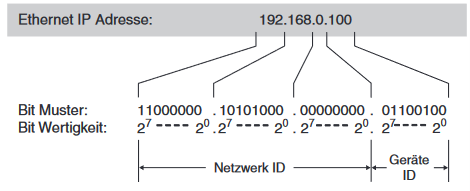
\includegraphics[width=0.70\linewidth]{./images/IP Adresse Aufbau.png}
   		\caption{IP-Adresse Aufbau \cite{hering2012elektrotechnik}} 
   		\label{fig:IP-Adresse}
   	\end{figure}
   	\\
   	\\
   	\textbf{Netzwerkarchitektur}\\
   	Während Netzwerke in ihrer Topologie, wie z.B. Bus, oder Stern-Topologie unterschieden werden können, kann auch eine Aufteilung nach Architekturtyp erfolgen. Neben der monolithischen Architektur und der Client-Server-Architektur gibt es Cloud-, Edge- und Fog-Computing. In der monolithischen Architektur existiert nur ein zentraler Rechner. An diesen werden externe Geräte angebunden, die selbst keine Rechenleistung aufweisen. Bei Cloud-, Edge- und Fog-Computing wird ein Teil der Netzwerktechnik an externe Organisationen ausgelagert. Eine externe Organisation kann ein Provider sein, der ein Server bereitstellt. \\
   	Im nachfolgenden soll die Client-Server-Architektur näher erläutert werden, da diese von Relevanz für diese Arbeit ist.
   	Bei der Client-Server-Architektur stellt der Client Anfragen an den Server, welche dieser beantwortet. Dieser Ablauf ist als Sequenzdiagramm in Abbildung \ref{fig:Sequenz Server-Client} dargestellt.\\
   	\begin{figure}[!ht]
   		\centering
   		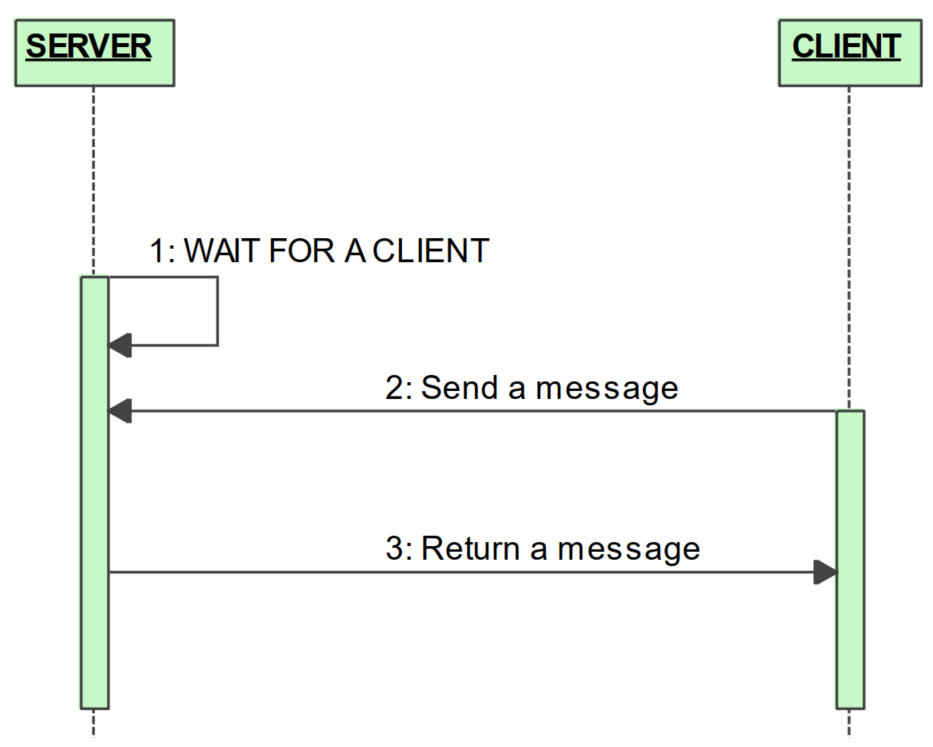
\includegraphics[width=0.50\linewidth]{./images/Sequenzdiagramm_Server_Client.png}
   		\caption{Sequenzdiagramm Server-Client-Architektur \cite{CS9_TCP}} 
   		\label{fig:Sequenz Server-Client}
   	\end{figure} \\   	
   	Charakteristisch für den Server ist dessen vergleichsweise hohe Rechenleistung, was es ermöglicht, dass mehrere Clients zeitgleich auf den Server zugreifen können. Veranschaulichen lässt sich dieses Prinzip mit dem Webbrowser, wie beispielsweise Google Chrome auf dem privaten Rechner. Dieser stellt den Client dar, welcher Anfragen an einen Webserver stellt, um aktuelle Daten passend zu seiner Anfrage zu erhalten. Auf dem Webserver wird beispielsweise ein Online-Shop verwaltet und mehrere Clients können zeitgleich auf diesen zugreifen. Das oben erwähnte Cloud-Computing basiert auf der Client-Server-Architektur, wurde jedoch nutzerfreundlicher gestaltet. \cite{IT-Sicherheit}
   	\label{sec:TCP/IP}
   	
   	\section{OPC/UA}
   	OPC UA (Open Platform Communication Unified Architecture) ist ein Protokoll zur Maschine-zu-Maschine-Kommunikation, aber auch zur Kommunikation zwischen SPS oder HMI (Human Interface) und Maschine. Es handelt sich hierbei um einen offenen und plattformunabhängigen Standard, welcher von der Open Platform Foundation (OPC) verwaltet wird. OPC UA basiert analog zu TCP/IP auf Ethernet und Internet. Es ist ebenso nicht echtzeitfähig. Das Kommunikationsprotokolls OPC UA ermöglicht eine vertikale und horizontale Kommunikation, da es die einzelnen Automatisierungsebenen verbindet. Somit kann von einem Roboter bis hin zur gesamten Fabriksteuerung alles verbunden werden, was OPC UA beliebt, um die Fabrik "Industrie 4.0" fähig zu machen. \cite{industrie40} \\
   	OPC UA basiert auf der Server-Client Architektur. Der OPC UA Server kann dann beispielsweise auf der SPS oder dem HMI (Human Interface) laufen und ein Roboter kann als OPC UA Client angebunden werden. Die Daten werden standardisiert und maschinenlesbar semantisch beschrieben, sodass herstellerübergreifende Kommunikation problemlos möglich ist. Sensordaten einer Maschine können dadurch an die Anlagensteuerung übertragen und visualisiert werden. OPC UA liefert dabei viele Vorteile: \cite{OPCUA}
   	\begin{itemize}
   		\item \textbf{Sicher:} IT-Sicherheit wurde bei der Entwicklung von OPC UA direkt mit eingeplant. Die Kommunikation und der Transport ist sicher und kann über Zugriffsrechte gesteuert werden.
   		\item \textbf{Plattformunabhängig:} Neben der Herstellerunabhängigkeit ist OPC UA unbhängig von der Programmiersprache, was es ermöglicht verschiedene Anlagen einfach zu verknüpfen.
   		\item \textbf{Einfach:} OPC UA ist auf Nutzerfreundlichkeit ausgelegt und das Festlegen von Kommunikationsprotokollen und der Aufbau von Nachrichten entfällt, sodass auch ohne Programmierkenntnisse eine Umsetzung möglich ist. 
   		\item \textbf{Big Data:} OPC UA ermöglicht einfaches Sammeln von Daten aus diversen Maschinen und von unterschiedlichsten Automatisierungsebenen. Hierdurch können sich umfangreiche Potentiale durch die Analyse der Daten ergeben und neue Geschäftsmodelle erschlossen werden. \\
   	\end{itemize}
   	Aufgrund dieser unterschiedlichsten Vorteile, wird OPC UA immer mehr im Bereich IoT und Industrie 4.0 eingesetzt. \cite{OPCUA}  \cite{industrie40}
   	
   	
   	\section{Stäubli-Roboter}
   	Stäubli ist ein in der Schweiz ansässiges Industrieunternehmen, welches in den Bereichen "Elektrische Verbindungen", "Fluidische Verbindungen","Textil" und "Robotik" tätig ist. Das Produktportfolio im Bereich Robotik umfasst Vier- und Sechsachs-Roboter, sowie kollaborative und mobile Roboter. \cite{StaubliUberUns}\\ Stäubli-Roboter sind nach IP 65 und IP 67 Staub- und Wasser- geschützt, wenn ein Arm mit Überdruckeinheit zum Einsatz kommt. Dies ermöglicht eine gründliche Reinigung aus Hygienezwecken und verhindert das Ansammeln von Staub im Roboter. Beispielsweise ist auch eine Reinigung mit Desinfektionsmittel oder Isopropylalkohol möglich. Zudem können die Roboter mit einem Lebensmittelverträglichem Öl eingesetzt werden. Stäubli-Roboter eignen sich daher insbesondere für Anwendungen in der Lebensmittel-, Pharma- und Medizin-Technik, in der viele andere Roboter die Hygieneanforderungen nicht erfüllen können. \cite{StaubliProduktubersicht}\\
   	\textbf{Roboter TX2 - 90}\\
   	Im Rahmen dieser Arbeit kommt der 6 Achs-Roboter TX2-90 zum Einsatz (vgl. Abbildung \ref{fig:TX90}). Dieser weist eine Tragkraft von 12 kg und eine Reichweite von 1000 mm auf. Die Wiederholgenauigkeit beträgt 0,03 mm und die maximale kartesische Geschwindigkeit 10,9 m/s. Der Roboter wiegt 114 kg und wird von der Robotersteuerung CS9 mit 2kVA gesteuert. Der Roboter ist für verschiedene, teils auch aggressive Reinigungsmittel geeignet, was für die Lebensmittelindustrie wichtig ist. Die Achsen können maximale Drehmomente zwischen 11 Nm (Achse 6) und 318 Nm (Achse 1) aufbringen.\\
   	Der Vorderarm des Roboters ist mit vier Magnetventilausgängen, von zwei 5/2-Wege-Magnetventilen versehen. Dies ermöglicht beispielsweise das Öffnen und Schließen eines Greifers.\\
   	Für den Roboter liegt ein Wartungsplan vor, welcher Wartungsarbeiten in unterschiedlichen Intervallen von monatlich bis 5-jährig vorsieht. Diese reichen von einfachen Sichtprüfungen und Bremsentests über Ölwechsel und Dichtungstausch bis hin zum Auswechseln von Achsen. \cite{X90}
   	\begin{figure}[!ht]
   		\centering
   		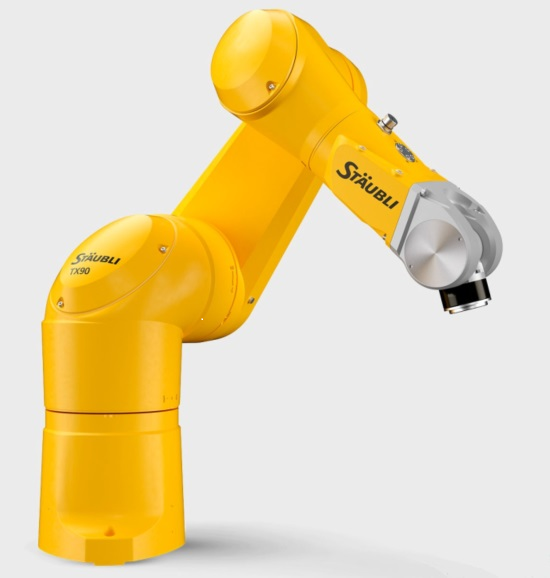
\includegraphics[width=0.50\linewidth]{./images/X90.png}
   		\caption{Stäubli TX2 - 90 \cite{X90}} 
   		\label{fig:TX90}
   	\end{figure}
   	\\
   	\subsection{Controller CS9}
   	Der CS9 Controller übernimmt die Steuerung und Versorgung des TX2 - 90 (vgl. Abbildung \ref{fig:CS9}).
   	\begin{figure}[!ht]
   		\centering
   		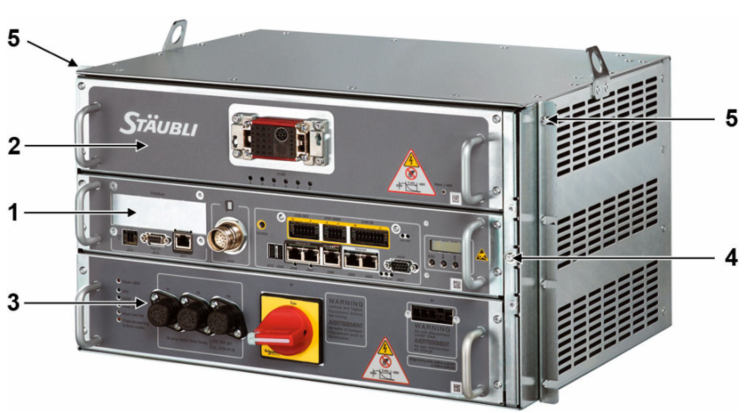
\includegraphics[width=0.70\linewidth]{./images/CS9.png}
   		\caption{Stäubli CS9 Controller \cite{CS9}} 
   		\label{fig:CS9}
   	\end{figure}
   	Der Computer-Einschub (1) beeinhaltet Karten, für die Sicherheitssteuerung, Bewegungssteuerung und die externe Kommunikation. Der Verstärker-Einschub (2) wandelt mit Hilfe von digitalen Achsverstärkern Bewegungsvorgaben in Motorströme um. Er beinhaltet zudem die Schnittstelle, an dem der Roboter angeschlossen wird. Der Stromversorgungs-Einschub (3) wandelt die Netzversorgungsspannung für die zuvor genannten Einschübe um und versorgt diese. Zudem existiert ein Anschluss für eine Antistatikmanschette (4), sowie Befestigungsmöglichkeiten (5).
   	\begin{figure}[!ht]
   		\centering
   		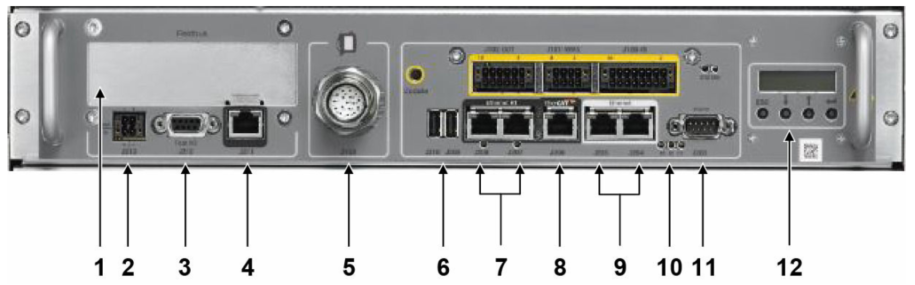
\includegraphics[width=0.70\linewidth]{./images/ComputerEinschub.png}
   		\caption{CS9 Controller Computer-Einschub \cite{CS9}} 
   		\label{fig:ComputerEinschub}
   	\end{figure}
   	Der Computer-Einschub (vgl. Abbildung \ref{fig:ComputerEinschub}) besitzt eine Vielzahl an Kommunikationsschnittstellen, die in der Tabelle nachfolgend dargestellt sind (vgl. Tabelle \ref{table:ComputerEinschub}).
   	\begin{longtable}{|p{1cm}|p{12cm}|}
   		\caption{CS9 Controller Computer-Einschub}
   		\label{table:ComputerEinschub}\\
   		\hline
   		Nr. & Bezeichnung  \\ [0.5ex] 
   		\hline
   		\endhead
   		1 & Feldbus, Option für PCIe-Karte  \\ 
   		2 & Anschluss für optionale externe 24 V Stromvesorgung  \\
   		3 & Schnelle Ein-/Ausgänge  \\
   		4 & EtherCAT Port (Reserviert) \\
   		5 & Anschluss Handbediengerät  \\
   		6 & USB-Ports \\  
   		7 & Echtzeit-Ethernet-Slave (EtherCAT, Sercos III, EtherNet/IP, PROFINET  \\ 
   		8 & EtherCAT-Master  \\ 
   		9 & Ethernet-Ports (1000 MBits/s und 100 MBits/s)  \\
   		10 & Status LEDs  \\ 
   		11 & serielle Verbindung RS232  \\
   		12 & Benutzerschnittstelle  \\  
   		\hline
   	\end{longtable}
   	 An den CS9 Controller kann kann ein Handbediengerät angeschlossen werden (5), was z.B.  manuelles Verfahren oder einfachere Programmier- und Konfigurationsarbeiten ermöglicht. Hervorzuheben ist zudem der Echtzeit-Ethernet-Slave-Anschluss (7), durch welchen die Steuerung z.B. über EtherCAT mit einer SPS verbunden werden kann. Zusätzlich steht ein EtherCAT-Master-Anschluss (8) zur Verfügung. Die CS9 ermöglicht es somit den Roboter als EtherCAT-Slave oder als EtherCAT-Master zu betreiben.\\
   	 Zudem stehen zwei Ethernet-Ports (9) zur Verfügung, was eine externe Kommunikation z.B. über TCP/IP ermöglicht. Die IP-Adresse der Ethernet-Ports kann frei konfiguriert oder automatisch vergeben werden. Als Dateiübertragungs-Serverprotokoll dient "FTPS+FTP". FTP wird als Standardeinstellung verwendet, während FTPS eine sichere Authentifizierung ermöglicht. \\
   	 Auf der CS9-Steuerung lassen sich sogenannte Sockets konfigurieren, welche eine TCP/IP oder eine UDP/IP - Kommunikation ermöglichen. Die Konfiguration kann dabei im Client oder Server-Modus erfolgen. \cite{CS9}
   	 
   	\subsection{Programmiersprache VAL3}
   	Die Programmierung des Roboters kann auf dem Handbediengerät erfolgen oder bevorzugt in der Stäubli Robotic Suite (SRS). In der SRS kann neben der Programmierung eine Simulation des Roboters inklusive 3D-Darstellung erfolgen, sodass die Programme direkt getestet werden können.\\
   	"VAL 3" ist eine höhere Programmiersprache und besitzt spezielle Steuerungsfunktionen für den Roboter zur Bewegungsteuerung und zur Ansteuerung von Ein-/Ausgängen.\\
   	\textbf{Programm} \\
   	In einer Applikation können mehrere Programme angelegt werden. Diese verhalten sich wie Funktionen und lassen sich aufrufen. Zur Ausführung der VAL3-Applikation wird standardmäßig das Prgoramm "start()" gestartet, welches vergleichbar mit einer "main-Funktion" ist. Von hier lassen sich wiederum andere Programme aufrufen. Bei Beendigung der Applikation wird das Programm "stop()" einmalig aufgerufen, um z.B. von dort Tasks zu beenden.
   	
   	
   	\section{Anlagensteuerung}
   	
   	
   
   	
   	\section{Bewertung}
   	In der Literatur wird meist das TCP Protokoll zur Datenübertragung eingesetzt, um die Korrektheit der Daten sicherzustellen. In \cite{groza2008using} kommt das Protokoll UDP zur Übertragung von Live-Kamera-Bildern zum Einsatz, da hier die Schnelligkeit über die Korrektheit zu stellen ist. Während in der Literatur z.B. in \cite{groza2008using} VPN zur IT-Sicherheit eingesetzt wird, kann dies im Rahmen des Projektes entfallen.
   	
	\newpage
	
	\chapter{Anforderungsdefinition}
	Die Aufgabenstellung und die grobe Anforderungsformulierung soll in diesem Kapitel mit Hilfe eines Lastenheftes in eine strukturierte Form gebracht werden. Das Lastenheft beschreibt, welche Funktionalitäten das zu entwerfende System aufweisen soll. Darüber hinaus kann das Lastenheft Rahmenbedingungen enthalten, wie z.B. zulässige Reaktionszeiten oder weitere Einschränkungen. Das Lastenheft wird in aller Regel vom Auftraggeber erstellt. Der Auftragnehmer beschreibt im Pflichtenheft durch welche Systemfunktionalitäten die Aufgaben erfüllt werden sollen und wie die Umsetzung technisch erfolgt. Das Lasten- und Pflichtenheft dient auch zur rechtlichen Absicherung der Vertragsparteien. Obwohl ein Lasten- und Pflichtenheft oft als Vertragsgrundlage entworfen wird und dies im Rahmen des Projektes nicht notwendig ist, soll ein Lastenheft eingesetzt werden. Dies ermöglicht es alle Anforderungen und Rahmenbedingungen zu berücksichtigen und diese im gesamten Projektverlauf im Blick zu behalten. Auf ein Pflichtenheft wird hingegen verzichtet. \cite{SoftwaretechnikBroy}
	Das Lastenheft wird in Muss- und Kann-Kriterien unterteilt. Während bei den Muss-Kriterien eine Erfüllung essentiell ist, stellen die Kann-Kriterien eine optionale Erweiterung dar, die dem System jedoch einen Mehrwert verschaffen.\\
	\begin{longtable}{|p{1cm}|p{10cm}|p{2cm}|}
		\caption{Lastenheft}
		\label{table:Lastenheft}\\
		\hline
		Nr. & Anforderung & Kann (K) / Muss (M) \\ [0.5ex] 
		\hline
		\endhead
		1 & Übertragung von Fehlermeldungen des Stäubli-Roboters an die Anlage & M  \\ 
		2 & Übertragung von beliebigen Daten des Stäubli-Roboters an die Anlage & M  \\
		3 & Übertragung von Daten z.B. Kameradaten von der Anlage an den Stäubli-Roboter & M  \\
		4 & Ausgabe der Roboterfehler auf der Anlagensteuerung in verständlicher Form (ausformuliert, Fehlercode genügt nicht) & M  \\
		5 & Funktionierende Feldbusverbindung zwischen Stäubli-Roboter und SPS & M  \\
		6 & Feldbus Kommunikation zwischen Stäubli-Roboter und SPS & M  \\  
		7 & Abspeichern der Fehler und der Daten in log-File & M  \\ 
		8 & Fehlerfreie und prozesssichere Kommunikation & M  \\ 
		\hline
		9 & Einsatz von mehreren Stäubli-Robotern zeitgleich soll möglich sein & K  \\
		10 & Vorgabe von der Anlagensteuerung, wie häufig Daten versendet werden sollen & K  \\ 
		11 & Visualierung der Daten & K  \\
		12 & Verwertung der Daten, um Warnungen oder ähnliches auszugeben & K  \\  
		\hline
	\end{longtable}
	
	\chapter{Konzeptionierung und Systementwurf}
	UML-Diagramm
	Anwendungsfälle definieren, Rahmenbedingungen identifizieren, Anforderungen aus Lastenheft
	 verfeinern
	 
	 Softwarekomponenten definieren und im Komponentendiagramm darstellen gemäß UML
	\section{Feldbus-Verbindung}
	
	\section{TCP/IP-Verbindung}
	
	\section{Datenverwertung}
	
	\begin{longtable}{|p{7cm}|p{3cm}|p{3cm}|}
		\caption{Verfügbare Daten}
		\label{table:Daten}\\
		\hline
		Daten & Zugriff & Verwendung  \\ [0.5ex] 
		\hline
		\endhead
		CPU battery test & D (CpuIO) & -  \\ 
		CPU overcurrent & D (CpuIO) & -  \\
		Fast memory state & D (CpuIO) & - \\
		CPU temperature & A (CpuIO) & Alarm, PM \\
		CPU board temperature & A (CpuIO) & Alarm, PM \\
		CPU fan speed & A (CpuIO) & Alarm, PM \\
		Free RAM & A (CpuIO) & - \\
		CFast memory remaining lifetime & A (CpuIO) & - \\
		\hline
		System management CPU usage & A (CpuUsage) & - \\
		Robot control CPU usage & A (CpuUsage) & - \\			
		Synchronous VAL 3 CPU usage & A (CpuUsage) & - \\
		Available CPU usage for VAL 3 processing& A (CpuUsage) & - \\
		User Fieldbuses CPU usage & A (CpuUsage) & - \\
		HMI CPU usage & A (CpuUsage) & - \\
		SRS connection CPU usage & A (CpuUsage) & - \\
		OPC-UA CPU usage & A (CpuUsage) & - \\
		CPU Load Score (higher is better)& A (CpuUsage) & - \\
		CPU Load Score (min) & A (CpuUsage) & - \\
		VAL 3 instructions per sequencing & A (CpuUsage) & - \\
		VAL 3 synr inst. per cyle (high priority) & A (CpuUsage) & - \\
		VAL 3 synr inst. per cyle (low priority) & A (CpuUsage) & - \\
		\hline
		Valve feedback (1.1, 1.2, 2.1, 2.2) & D (DsiIO) & - \\
		Axis brake feedback (1-6) & D (DsiIO) & - \\
		Error on valves outputs & D (DsiIO) & Alarm \\
		Error on brakes outputs & D (DsiIO) & Alarm \\
		Error on safe digital inputs & D (DsiIO) & Alarm \\
		DSI non-reduced brake supply voltage undershoot & D (DsiIO) & Alarm \\
		DSI reduced brake supply voltage undershoot & D (DsiIO) & Alarm \\
		DSI logic supply voltage undershoot & D (DsiIO) & Alarm \\
		DSI overtemperature & D (DsiIO) & Alarm \\
		\hline
		DSI board tempereature & A (DsiIO) & Alarm, PM \\
		Axis motor temperature (1-6) & A (DsiIO) & Alarm, PM \\
		Axis encoder temperature (1-6) & A (DsiIO) & Alarm, PM \\
		DSI state & A (DsiIO) & - \\
		DSI error code & A? (DsiIO) & ? Grau? Alarm \\
		Arm operation counter & A (DsiIO) & - \\
		\hline
		safe Input state (0-7) & D (DsiIoSafe) & - \\
		\hline
		Fast Input (1-2) & D (FastIO) & - \\
		Fast Output (1-2) & D (FastIO) & - \\
		\hline
		Power unit identification (bit 1-3) & D (PSIO) & - \\
		Main power state & D (PSIO) & - \\
		Internal bus voltage state & D (PSIO) & - \\
		Power unit internal temperature state & D (PSIO) & - \\
		24V state & D (PSIO) & - \\
		Buckfull mode feedback & D (PSIO) & - \\
		Memorize a power dropout & D (PSIO) & - \\
		\hline
		Brake test warning & D (Rsi9IO) & Alarm \\
		Brake test successful & D (Rsi9IO) & - \\
		Temperature of RSI board & A (Rsi9IO) & Alarm, PM \\
		Error Code of RSI board & A? (Rsi9IO) & ?Grau? Alarm \\
		\hline
		STARC board temperature & A (StarcIO) & Alarm, PM \\
		Axis drive case temperature (1-6) & A (StarcIO) & Alarm, PM \\
		Motor Winding Temperature (1-6) & A (StarcIO) & Alarm, PM \\
		Axis drive junction temperature (1-6) & A (StarcIO) & Alarm, PM \\		
		\hline
		Geschwindigkeit Endmanipulator & getSpeed(...) & - \\
		Schleppfehler Achsen 1-6 & getPositionErr()  & - \\
		Drehmoment Achsen 1-6 & getJointForce(...)  & - \\
		Bewegungsauftrag und Fortschritt & getMoveld()  & - \\
		Konfiguration des Roboters & getVersion(...)  & - \\
		Stromversorgung bei Stillstand abschalten & hibernateRobot()  & - \\
		Systemereignisse &getEvents(...)  & - \\
			
	\end{longtable}
	Durch die Verfügbarkeit von Roboterdaten ergeben sich Nutzungspotentiale, wie z.B.:
	\begin{itemize}
		\item \textbf{Überwachung und Alarm:} Bei Überschreiten von Schwellwerten oder bei Fehlermeldungen Alarm auslösen
		\item \textbf{Predictive Maintenance:} Vorhersagen treffen, wann Wartung erfolgen soll, um Ausfälle vorbeugend zu verhindern.
		\item \textbf{Datenarchivierung und Compliance:} Datenspeicherung für Schadensfall oder gesetzliche Gewährleistung
		\item \textbf{Trendanalyse:} Muster und Tendenzen in den Daten erkennen
	\end{itemize}
	
 	Prinzipiell lassen sich alle verfügbaren Daten sammeln, visualisieren und auswerten. Bei einigen dieser Daten wie z.B. des freien RAM-Speichers ist der daraus entstehende Nutzen beschränkt.	Mittels Brainstorming wurden verschiedene Anwendungsszenarien ausgedacht, im nachfolgenden sollen jedoch nur die sinnvollsten hiervon vorgestellt werden.\\
 	\textbf{Temperaturen}\\
 	Neben der Temperatur von verschiedenen Computer-Chips und Platinen, wie z.B. CPU, CPU-Platine DSI-Platine, RSI-Platine und STARC-Platine sind verschiedene Temperaturwerte von den Antrieben abrufbar. Hier sind die Temperaturen der Motoren, Encoder, Antriebsgehäuse,  Antriebswicklungen und  Steuergeräte zu nennen. Diese Daten können sowohl zur Überwachung als auch zur Predictive Maintenance verwendet werden. Bei Überschreiten eines Grenzwertes kann ein Alarm bzw. eine Warnung ausgegeben werden. Da von Seiten des Herstellers keine zulässigen Grenzwerte vorgegeben sind, müssen die aufgezeichneten Messwerte unter Berücksichtigung von Schwankungen analysiert werden und Grenzwerte festgelegt werden, ab welchen Werten das Verhalten nicht mehr als "normal" angesehen werden kann. Die Dynamik von Temperaturen ist im Allgemeinen relativ gering, da sich die Materialien aufgrund ihrer Wärmekapazität erst aufheizen müssen. Aus diesem Grund ist das Übertragen von den Temperaturwerten in vergleichsweise großen Abständen zulässig z.B. alle 15 Sekunden. Im Falle eines technischen Defektes wäre eine möglichst frühe Warnung wünschenswert, jedoch ist die Zeit bis ein Techniker den Alarm wahrnimmt und entsprechende Aktionen starten kann vergleichsweise groß, weshalb dieser Anwendungsfall kein höhere Übertragungsrate rechtfertigt. Da die Genauigkeit von vielen Temperatursensoren nur im Bereich von 0,5K liegt und sehr genaue Temperaturwerte keinen zusätzlichen Mehrwert bieten, ist eine Übertragung der Temperaturen ohne Nachkommastellen ausreichend. Dadurch lässt sich ein Temperaturwert problemlos mit einem einzelnen Byte (Werte zwischen 0 und 255°C) übertragen.\\
 	\textbf{Error-Meldungen}\\
 	Von dem Stäubli-Roboter werden einige Fehlermeldungen erfasst, wie von den Ventil und Brems-Ausgängen, den digitalen Sicherheits-Eingängen, des DSI-Chip, RSI-Chip und Bremsentests. Ebenso werden "DSI non-reduced brake supply voltage undershoot",  "DSI reduced brake supply voltage undershoot", "DSI logic supply voltage undershoot" und "DSI overtemperature" erfasst. Error-Meldungen wie diese sollen als Alarm bzw. Fehlermeldung ausgegeben werden. Ebenso ist ein Dokumentieren sinnvoll, um bei Ausfällen oder Defekten die Ursachensuche zu erleichtern. Jeder Fehler kann als Wert 1 oder 0 dargestellt werden, weshalb je Fehlermeldung ein Bit genügt. Alle Error-Meldungen lassen sich somit über 2 Bytes abbilden.\\
 	\textbf{Schleppfehler}\\
 	Der Schleppfehler entspricht der Abweichung zwischen Soll-Position und Ist-Position jeder einzelnen Achse. Ein herausstechend großer Schleppfehler kann auf Probleme mit der Steuerung, den Motoren, den Encoder oder den Achsen selbst hinweisen. Eine genaue Eingrenzung ist auf Basis der gegebenen Daten nicht möglich, jedoch ist eine Warnung sinnvoll. Zur Ermittlung der Grenze, bei deren Überschreiten eine Warnung ausgegeben werden soll, können aufgezeichnete Daten unter Berücksichtigung von Schwankungen herangezogen werden. Der Schleppfehler muss sehr regelmäßig erfasst werden, um die kontinuierliche Bewegung best möglichst abzubilden.\\
 	\textbf{Drehmoment Achsen}\\
 	Das Drehmoment der einzelnen Achsen ändert sich kontinuerlich während der Bewegung. Durch das Vergleichen der Drehmomente mit einer Referenzfahrt können  Auffälligkeiten entdeckt werden. Schleichend zunehmende Momente deuten z.B. auf fehlende Schmierung oder Lagerdefekte hin. Abrupt zunehmende Momente können durch ein Festhängen oder einen Crash verursacht werden. Eine Dokumentation der Abweichungen ist sinnvoll, um aus Gewährleistungsgründen unsachgemäße Verwendung z.B. durch einen Crash nachzuweisen. Analog zum Schleppfehler müssen auch die Drehmomente sehr kontinuierlich erfasst werden.\\
	\textbf{Sytemereignisse}\\
	Ereignisse, die von der Steuerung festgestellt werden, wie z.B. Fehlermeldungen oder das Einschalten der Energieversorgung für die Achsen werden in einer system-log-Datei aufgezeichnet. Sie lassen sich in die Schweregrade "Info", "Warning", "Error" und "Critical" unterteilen. Das Auslesen der Systemereignisse kann mit dem Befehl "getEvents" erfolgen. Diese sollen beim Auftreten sofort über TCP/IP übertragen werden.
	\newpage
	
	\section{WPF und GUI}
	
	\chapter{Design und Implementierung}
	Design: Vergleich von Lösungsbausteinen (z.B. Vergleich Softwarebibliotheken) und Auswahl) auf Basis von Anforderungen und Recherche. Wissenschaftliche Bewertungskriterien nötig. Harvey-Diagramm.
	
	Neben grundlegenden Entwurfsentscheidungen wird die Beschreibung einzelner Komponenten detailiert. Für komplexe Komponenten UML-Klassendiagramm
	Definition Schnittstelle zwischen den Komponenten und Kommunikation in Form von Sequenzdiagramm
	
	
	Implementierung
	- Programmierung erfolgt gemäß den in Softwarespezifikation und entwurf festgelegten Randbedingungen, Kommentierung von Source Code ist essentiell. Gemäß bestehenden Standards (z.B. xdoc)
	- Generierung einer HTML-Hilfe aus den Kommentaren des Source-Codes z.b. durch Doxygen
	- Entwicklung erfolgt unter Git
	- Einheitliche Konventionen für das Schreiben des Quellcodes: Coding Conventions!
	\section{Stäubli-Roboter in VAL3}
	
	\subsection{EtherCAT}
	
	\subsection{TCP/IP}
	Für die Implementierung der TCP/IP-Verbindung auf dem Controller des Stäubli-Roboters muss in der SRS eine Socket-Verbindung angelegt werden. Hierzu wird in der E/A-Verwaltung ein Client angelegt, welcher die IP-Adresse und den Port des Servers zugewiesen bekommt. Darüber hinaus wird ein sogenannter Timeout von 0 s gesetzt. Bei einem Timeout von 0 wird auf den Vorgang, welcher ein Lesen oder Schreiben sein kann gewartet. Bei einem Timeout kleiner 0 wird hingegen nicht bis zur Ausführung des Vorgangs gewartet. Be einem Timeout größer 0 wird hingegen eine gewisse Zeit gewährt, bis zu dieser der Timeout durchgeführt werden kann. Die Nachricht soll in diesem Fall jedoch direkt gelesen oder geschrieben werden, weshalb kein Spielraum im Rahmen des Timeouts gewährt wird. \cite{VAL3} Die Socket-Verbindung wird als E/A-Verbindung in VAL3 betrachtet, weshalb eine globale Variable mit dem Namen des Clients angelegt werden kann und hierüber auch gelesen und beschrieben werden kann. Die Socket-Verbindung wird nur dann erstellt, wenn sie ihm Rahmen des Programmablaufs z.B. durch die Befehle sioSet und sioGet benötigt wird. Der Client versucht dann eine Verbindung zum Server aufzubauen.   usepackage{ffcode}\\
	num sioGet(sio siInput, num\& nData[])\\
	Diese Funktion schreibt ein gelesenes Zeichen oder einen gelesen Array von Zeichen von siInput in das Array nData. Als Rückgabewert dient die Anzahl der gelesenen Zeichen.	
	num sioSet(sio siOutput, num\& nData[]) \\
	Mit dieser Funktion kann in VAL3 die zu übermittelnde Nachricht nData versendet werden, indem der E/A-Verbindung siOutput die Nachricht zugewiesen wird. Zurückgegeben wird die Anzahl der geschriebenen Zeichen oder "-1" im Falle des Timeouts. \\
	Das Versenden von Nachrichten erfolgt über einen Byte-Array, das heißt durch die Aneinanderreihung mehrerer Bytes. Folglich muss die zu versendete Nachricht in einen Byte-Array umgewandelt werden und beim Empfangen muss der Byte-Array interpretiert werden.\\
	num toBinary(num nValue[], num nValueSize, string sDataFormat, num\& nDataByte[])\\
	Diese Funktion wandelt einen numerischen Wert, welcher das Datenformat sDataFormat besitzt in einen Byte-Strom und speichert diesen im Array nDataByte. Über das Datenformat wird beispielsweise angegeben ob es sich um einen Gleitkommawert handelt, ob ein Vorzeichen vorliegt und ob das Little-Endian oder das Big-Endian-Format angewandt wird. Mit nDataSize kann die Anzahl der zu kodierenden Zeichen beschränkt werden.\\
	num fromBinary(num nDataByte[], num nDataSize, string sDataFormat, num\& nValue[])\\
	Umgekehrt ermöglicht diese Funktion, einen empfangen Byte-Array in numerische Werte zu konvertieren. Das Ergebnis im Datenformat nDataFormat wird in nValue gespeichert. Die Anzahl der zu decodierenden Bytes wird festgelegt durch nDataSize, wenn nicht alle Bytes des Eingangs-Array nDataByte decodiert werden sollen.
	
	\section{.NET in C\#}
	
	
	\subsection{TCP/IP}
	
   	\subsection{Datenverwertung und Visualisierung}
   	
   	
   	\chapter{Validierung}
   	
   	\chapter{Ausblick und Fazit}
   	
   	\backmatter
   	
   	
   	\cleardoublepage
   	\listoffigures
   	\cleardoublepage
   	\listoftables
   	\cleardoublepage
   	
   	\cleardoublepage
   	\printbibliography
   	
   	% Acronyms   	
   	% Appendix, if needed:
   

\end{document}